\begin{frame}
\frametitle{Aufgabe 2}
\framesubtitle{Messung 1: einfache Parallelschaltung}
    Es soll eine einfache Parallelschaltung untersucht werden.\\
    Parallelschaltung $1k\Omega$ und $100k\Omega$
    \begin{figure}[H]
    \begin{center}
            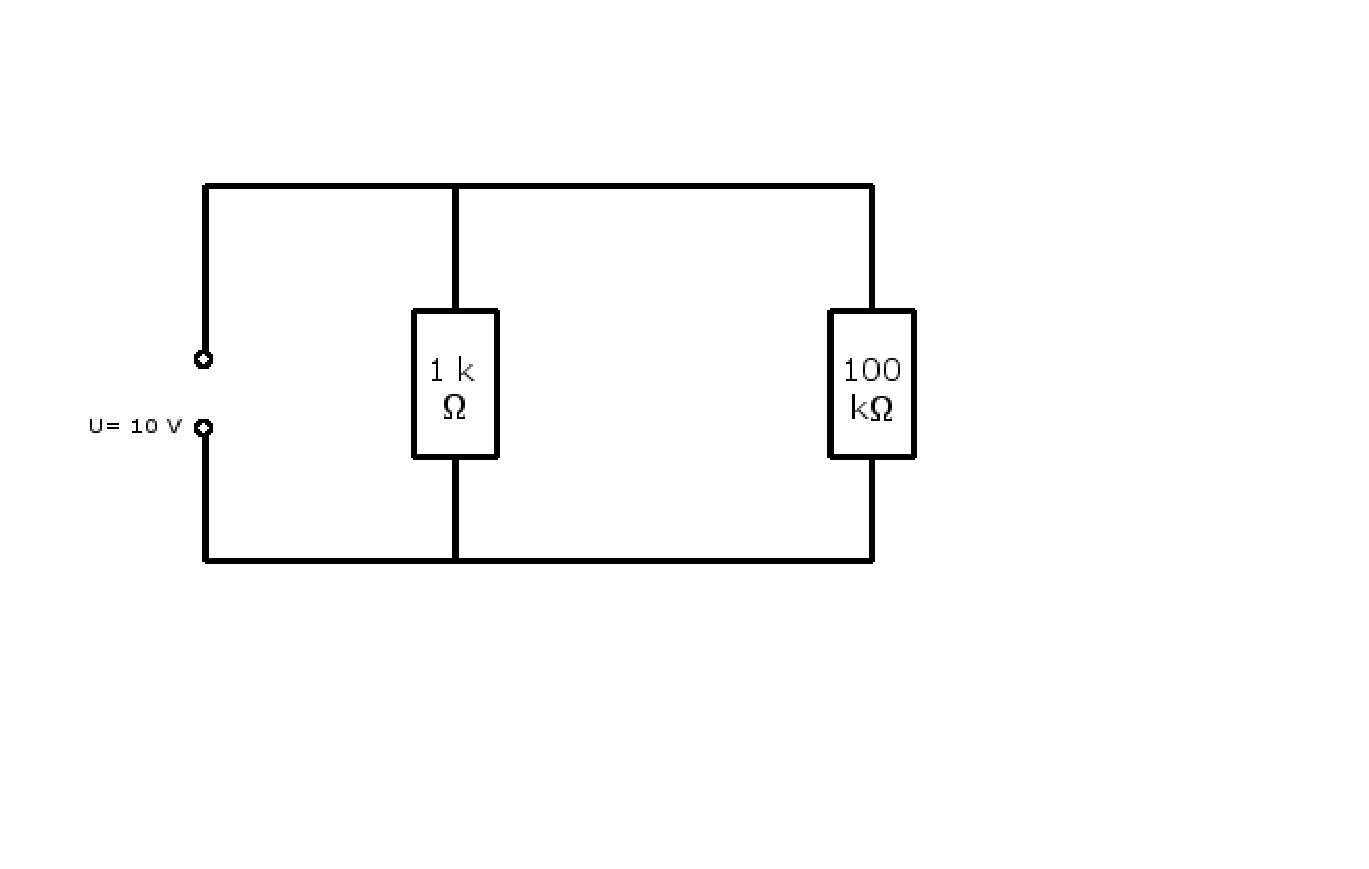
\includegraphics[scale=0.60]{./img/parallelschaltungfrei.eps}
    \end{center}
    \end{figure}
    
\end{frame}
\begin{frame}
\frametitle{Aufgabe 2}
\framesubtitle{Messung 1: einfache Parallelschaltung}
    Erwarteter Widerstand: $R_{ges} = 990 \Omega$
    \hline
    \begin{tabular}{c| c c|c|c}
                        & $I/mA$ & $U/V$ & $R/\Omega$ berechnet& $R/\Omega$ gemessen \\
                        \hline
        Gesamtschaltung & 10.19&10&981.4& \\
        Widerstand $1$  & 10.09&10&991&991.9 \\
        Widerstand $2$  & 0.1&10&10000&98940 
    \end{tabular}
    $\rightarrow$ Werte stimmen innerhalb des Toleranzbereichs mit Rechnung überein.
\end{frame}

\begin{frame}
\frametitle{Aufgabe 2}
\framesubtitle{Messung 2: geringer Gesamtwiderstand}
    Es soll eine Schaltung mit $R_{ges} \leq 800 \Omega$ untersucht werden.\\
    Parallelschaltung $2 \times 1k\Omega$ 
    \begin{figure}[H]
    \begin{center}
            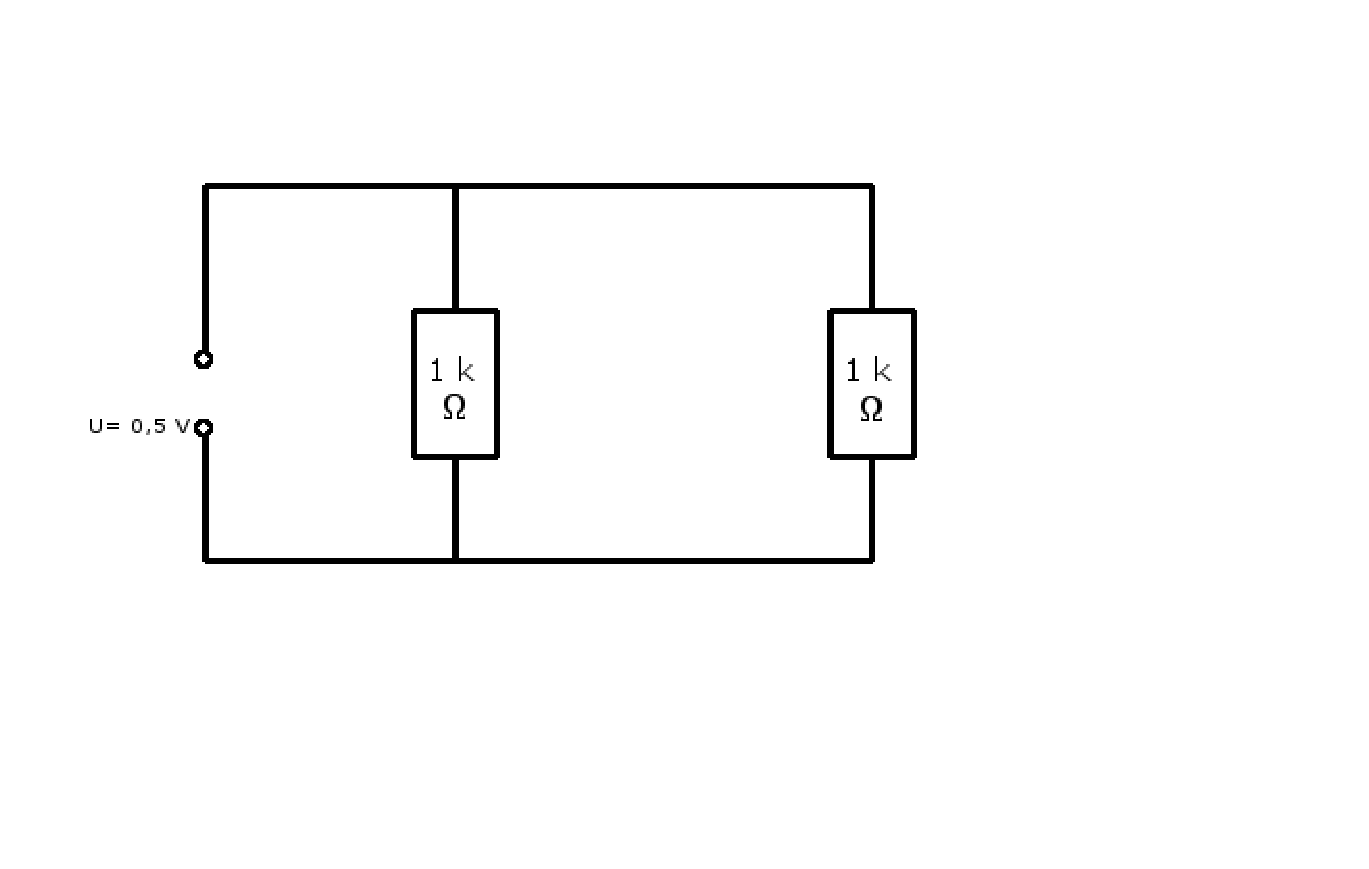
\includegraphics[scale=0.6]{./img/parallelschaltung.eps}
    \end{center}
    \end{figure}
    
\end{frame}
\begin{frame}
\frametitle{Aufgabe 2}
\framesubtitle{Messung 2: geringer Gesamtwiderstand}
    Erwarteter Widerstand $R_{ges} = 500\Omega$
    \hline
    \begin{tabular}{c| c c|c|c}
    & $I/mA$ & $U/V$ & $R/\Omega$ berechnet& $R/\Omega$ gemessen \\
            \hline
    Gesamtschaltung & 0.72&0.5&694.4& \\
    Widerstand $1$  & 0.42&0.5&1190&0.992 \\
    Widerstand $2$  & 0.42&0.5&1190&0.991 \\
    \end{tabular}
    $\rightarrow$ $I$-Werte liegen zu niedrig 
\end{frame}

\begin{frame}
\frametitle{Aufgabe 2}
\framesubtitle{Messung 3: hoher Gesamtwiderstand}
    Es soll eine Schaltung mit $R_{ges} \geq 8M \Omega$ untersucht werden.\\
    Reihenschaltung $2 \times 4.7M\Omega$ 
    \begin{figure}[H]
    \begin{center}
            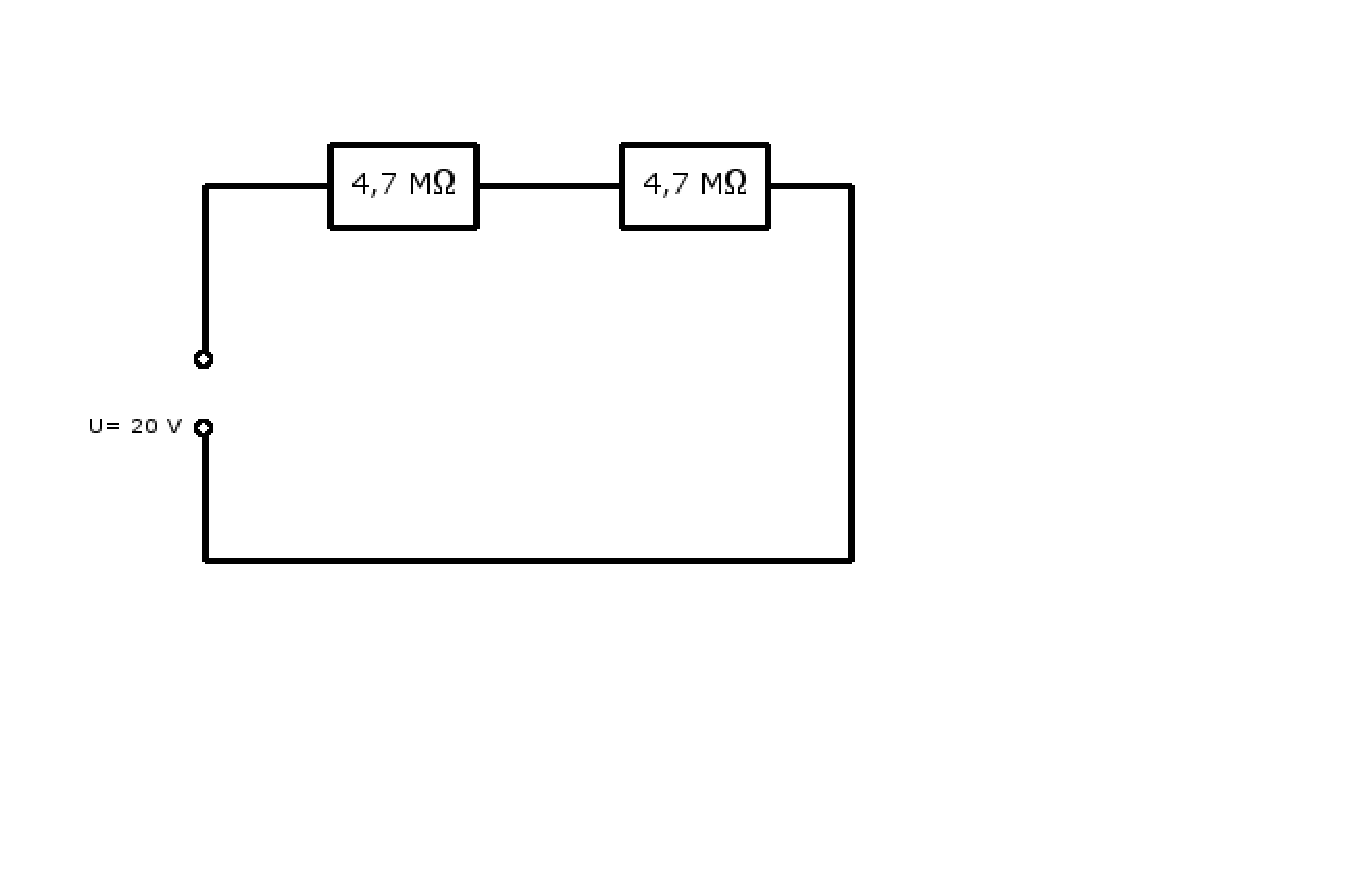
\includegraphics[scale=0.6]{./img/reihenschaltung.eps}
    \end{center}
    \end{figure}
    
\end{frame}
\begin{frame}
\frametitle{Aufgabe 2}
\framesubtitle{Messung 3: hoher Gesamtwiderstand}
    Erwarteter Widerstand $R_{ges} = 9.4 M\Omega$
    \begin{tabular}{c| c c|c|c}
    \hline
    & $I/\mu A$ & $U/V$ & $R/M\Omega$ berechnet& $R/M\Omega$ gemessen \\
                \hline
    Gesamtschaltung & 2.1&20&9.5&\\
    Widerstand $1$  & 2.1&8.12&3.9&4.7 \\
    Widerstand $2$  & 2.1&8.0&3.8&4.7  \\
    \end{tabular}
    $\rightarrow$ $U$-Werte zu niedrig \\
\end{frame}
\begin{frame}
\frametitle{Aufgabe2}
\framesubtitle{Messung3: HI-Z}
Nach Umstellen des DMM auf "HI-Z":
    \begin{tabular}{c| c c|c|c}
    \hline
    & $I/\mu A$ & $U/V$ & $R/M\Omega$ berechnet& $R/M\Omega$ gem. \\
                \hline
    Gesamtschaltung & 2.1&20&9.5&\\
    Widerstand $1$  & 2.1&10.0&4.8&4.7 \\
    Widerstand $2$  & 2.1&9.97&4.7&4.7  \\
    \end{tabular}
    $\rightarrow$ korrigierte $U$-Werte liefern erwarteten Widerstand 
\end{frame}
\begin{frame}
\frametitle{Aufgabe 2}
\framesubtitle{Erklärung}
    \begin{itemize}
        \item niedriger Widerstand: Innenwiderstand nicht sehr viel kleiner als
        Gesamtwiderstand: DMM kein  ideales Strommessgerät \\
        Innenwiderstand beeinflusst Messung
        \item hoher Widerstand:  Innenwiderstand nicht sehr viel größer als
        Gesamtwiderstand:  DMM kein  ideales Spannungsmessgerät \\
     \end{itemize}
     $\rightarrow$ Innenwiderstand beeinflusst Messung
     \begin{itemize}
        \item HI-Z: Innenwiderstand wird auf $10G\Omega$ gesetzt $\rightarrow$
        Innenwiderstand wieder sehr viel großer als Gesamtwiderstand
    \end{itemize}
    Messung wird an Randbereichen ungenauer: Für gute Ergebnisse muss man das
    Messgerät berücksichtigen.
\end{frame}


%\begin{tabular}{c| c c|c|c}
%                    & $I/mA$ & $U/V$ & $R/\Omega$ berechnet& $R/\Omega$ gemessen \\
%                    \hline
%    Gesamtschaltung & &&& \\
%    Widerstand $1$  & &&& \\
%    Widerstand $2$  & &&& 
%\end{tabular}
